% SPDX-License-Identifier: CC-BY-SA-4.0
%
% Copyright (c) 2020 Philipp Le
%
% Except where otherwise noted, this work is licensed under a
% Creative Commons Attribution-ShareAlike 4.0 License.
%
% Please find the full copy of the licence at:
% https://creativecommons.org/licenses/by-sa/4.0/legalcode

\chapter{Digital Signal Processing}

\begin{refsection}
	
At this point we have learnt about:
\begin{itemize}
	\item Mixing \ac{RF} signals down to the baseband using IQ demodulators. And vice verse, mixing baseband signals up to \ac{RF} using IQ modulators.
	\item Digitizing these analogue baseband signals.
\end{itemize}

The digitized baseband signal is now processed digitally.
\begin{itemize}
	\item There are no analogue baseband processing hardware components like in a traditional radio.
	\item The baseband processing is digital after the \ac{ADC}. The time-discrete and value-discrete baseband is processed by:
	\begin{itemize}
		\item Software: A \ac{CPU} executes a software processing the digital baseband signal.
		\item Digital hardware: Digital hardware components (like \ac{PLD}/\ac{FPGA}, \ac{ASIC}) process the digital baseband in logic gates.
		\item Hybrid: A part of signal processing is done in digital hardware. Another part is done in software.
	\end{itemize}
\end{itemize}

\textbf{Benefits and drawbacks of digital hardware}:
\begin{itemize}
	\item The signal processing is parallel. The logic gates operate parallelly.
	\item Large amount of data can be processed (e.g. high- sampling rate).
	\item The logic gates are programmed (\ac{PLD}, \ac{FPGA}) or statically configured during manufacturing (\ac{ASIC}). Especially, \acp{ASIC} cannot be reconfigured later. An update is not possible.
	\item Digital hardware is suitable of accomplishing the tasks of lower protocol layers, especially layer 1 (physical layer). The hardware design becomes difficult for higher protocol layers, requiring sequential processing.
\end{itemize}

\textbf{Benefits and drawbacks of software}:
\begin{itemize}
	\item A software is a set of instructions, sequentially executed by a \ac{CPU}.
	\item Some extent of parallelism can be achieved by multitasking and multiprocessing.
	\item The lack of parallelism limits the capability of processing large amounts of data.
	\item Specialized \acp{DSP} offer instructions to speed up some processing tasks requiring intensive, parallel calculations (vector instructions).
	\item Software is flexible. Software can be easily updated. So the program can be adapted to fit new applications.
	\item Usually, a software includes higher protocol layers, which tend to require sequential processing.
\end{itemize}

\begin{fact}
	Implementing large amounts of the signal processing digitally in software is called \acf{SDR}.
\end{fact}

\textbf{Hybrid technologies:}
\begin{itemize}
	\item A good trade-off is to split the signal processing between digital hardware and software.
	\item Hardware manufactures may implement general signal processing tasks (filtering, resampling, etc.) in hardware and offer an interface to the software.
	\item The signal processing is fast, while the software can be updated and re-configure the hardware if required.
	\item Hybrid technologies are not as flexible as \ac{SDR}, require less \ac{CPU} processing power, which makes them cheaper and reduces the power consumption.
	\item The digital communication system is flexible and can be easily adapted to meet new requirements and fit new applications, without the need to change the hardware. Hardware changes would require costs for development, production and installation.
	\item Software updates can be easily deployed. This significantly reduces the maintenance costs.
\end{itemize}

\begin{fact}
	Power consumption is an important property. In many \ac{IOT} applications, the devices must have a battery lifetime of several years. Maintenance tasks (and therefore costs) like changing the battery would make those applications infeasible.
\end{fact}

\section{Digital Systems}

So far, we have learnt about analogue systems:
\begin{itemize}
	\item Filters
	\item Mixers
	\item Samplers
	\item Amplifiers
\end{itemize}

All analogue systems can be transferred to the time-discrete domain and be implemented there. The z-transform is used to describe and analyse digital systems.
\begin{figure}[H]
	\centering
	\begin{tikzpicture}
		\node[draw, block] (System) {System\\ $\underline{h}[n]$};
		\draw[<-o] (System.west) -- ++(-2cm, 0) node[above, align=center]{Input signal\\ $\underline{x}[n]$};
		\draw[->] (System.east) -- ++(2cm, 0) node[above, align=center]{Output signal\\ $\underline{y}[n]$};
	\end{tikzpicture}
	\caption{A digital system with input and output}
\end{figure}

The \index{transfer function!time-discrete systems} \textbf{transfer function} $\underline{H}(\underline{z})$ of the system is:
\begin{equation}
	\underline{H}(\underline{z}) = \frac{\underline{Y}(\underline{z})}{\underline{X}(\underline{z})} = \frac{\mathcal{Z}\left\{\underline{x}[n]\right\}}{\mathcal{Z}\left\{\underline{y}[n]\right\}}
\end{equation}

Its time-domain representation is the \index{impulse response!time-discrete systems} \textbf{impulse response} $\underline{h}[n]$.
\begin{subequations}
	\begin{align}
		\underline{H}(\underline{z}) &= \mathcal{Z}\left\{\underline{h}[n]\right\} \\
		\underline{h}[n] &= \mathcal{Z}^{-1}\left\{\underline{H}(\underline{z})\right\}
	\end{align}
\end{subequations}

The impulse response is directly obtained as the system's output when an ideal impulse (Kronecker delta\footnote{The Kronecker delta is the time-discrete variant of the Dirac delta function}) is applied to the system's input.
\begin{equation}
	\begin{split}
		\underline{y}[n] = \underline{h}[n] &= \underline{h}[n] * \underbrace{\delta[n]}_{= 1 \text{ for } n=0, \; 0 \text{ else}.} \\
		\underline{Y}(\underline{z}) = \underline{H}(\underline{z}) &= \underline{H}(\underline{z}) \cdot \underbrace{\mathcal{Z}^{-1}\left\{\delta[n]\right\}}_{=1} \\
	\end{split}
\end{equation}

\begin{remark}
	The z-transform applies to both value-discrete and value-continuous signals, as long as they are time-discrete. However, in this chapter we are are already in the digital domain, i.e., time-discrete and value-discrete.
\end{remark}

\begin{remark}
	While being in the analogue domain, the signals were always assumed to be real-valued in the time-domain. The reason was that they must be able to exists as a physical signal. Now, the time-domain signals may be complex-valued. In the digital domain, the signals are just numbers. Refer to the IQ modulation and modulation of complex baseband signals (Chapter 5) for details.
\end{remark}

\begin{remark}
	Digital signals are always band-limited.
	\begin{itemize}
		\item Please remember that signals can only be processed up to a certain bandwidth with is related to the sampling rate (Shannon-Nyquist sampling theorem, repeating replica of the spectrum).
		\item Higher bandwidth baseband signals require a higher sampling rate and more processing power.
	\end{itemize}
\end{remark}

\section{Digital Filters}

Like analogue filters, digital filters eliminate undesired bands and only let desired ones pass. There are:
\begin{itemize}
	\item \acf{LPF},
	\item \acf{HPF},
	\item \acf{BPF}, and
	\item \acf{BSF}.
\end{itemize}

\begin{remark}
	This section considers the general theory of filters. The very interesting topic of the filter design is unfortunately beyond the scope of this lecture. There are dedicate lectures on this topic. In addition, you will find plenty of literature and other resources. For practical application, you will find filter design software\footnote{For example, the ``numpy'' and ``scipy'' Python packages provide nice filter design and analysing tools for both scientific and engineering use. It's free software.}.
\end{remark}

\subsection{Infinite Impulse Response Filters}

Chapter 2 showed the ideal filter shapes in the frequency domain. These shapes can be resembled in digital filters.

However, the filter is implemented in the time-domain.

\begin{figure}[H]
	\centering
	\begin{circuitikz}
		\foreach \x in {0,1,2}{
			\draw (4,{-3*\x}) node[adder](AddA\x){};
			\draw (1,{-3*\x}) to[twoport,t=$z^{-1}$,>,*-] ++(0,-3);
			\draw (1,{-3*\x}) to[amp,l=$\underline{b}_\x$,>,-] (AddA\x.west);
			\draw (AddA\x.west) node[inputarrow]{};
		}
	
		\draw (6,0) node[adder](AddB0){};
		\draw (9,0) to[twoport,t=$z^{-1}$,>,*-] ++(0,-3);
		\draw (AddB0.east) -- (9,0);
		\foreach \x in {1,2}{
			\draw (6,{-3*\x}) node[adder](AddB\x){};
			\draw (9,{-3*\x}) to[twoport,t=$z^{-1}$,>,*-] ++(0,-3);
			\draw (9,{-3*\x}) to[amp,l=$\underline{a}_\x$,>,-] (AddB\x.east);
			\draw (AddB\x.east) node[inputarrow,rotate=180]{};
		}
	
		\draw[-latex] (AddA1.north) -- (AddA0.south);
		\draw[-latex] (AddA2.north) -- (AddA1.south);
		\draw (1,-9) to[amp,l=$\underline{b}_3$] ++(3,0) -| (AddA2.south);
		\draw (AddA2.south) node[inputarrow,rotate=90]{};
		
		\draw[-latex] (AddB1.north) -- (AddB0.south);
		\draw[-latex] (AddB2.north) -- (AddB1.south);
		\draw (9,-9) to[amp,l=$\underline{a}_3$] ++(-3,0) -| (AddB2.south);
		\draw (AddB2.south) node[inputarrow,rotate=90]{};
		
		\draw[-latex] (AddA0.east) -- (AddB0.west);
		
		\draw (2.5,-10.5) node[below,align=center]{\textbf{Feed-forward}};
		\draw (7.5,-10.5) node[below,align=center]{\textbf{Feed-back}};
		
		\draw[o-] (0,0) node[left, align=right]{Input signal\\ $\underline{x}[n]$} -- (1,0);
		\draw[-latex] (9,0) -- (10,0) node[right, align=left]{Output signal\\ $\underline{y}[n]$};
		
		\draw[dashed] (5,-2.4) -- (5,-3.6) -- (0,-3.6) -- node[midway,left,align=right]{Filter tap} (0,-2.4) -- cycle;
	\end{circuitikz}
	\caption{Block diagram of an example \acs{IIR} filter}
	\label{fig:ch06:iir_filt}
\end{figure}%
\nomenclature[Bd]{\begin{circuitikz}[baseline={(current bounding box.center)}]\draw (0,0) to[twoport,t=$z^{-1}$,>] (2,0);\end{circuitikz}}{Delay element}%
\nomenclature[Ba]{\begin{circuitikz}[baseline={(current bounding box.center)}]\node[adder](){};\end{circuitikz}}{Adder}

Figure \ref{fig:ch06:iir_filt} shows an example filter. The block diagram has following digital components:
\begin{itemize}
	\item \begin{circuitikz}[baseline={(current bounding box.center)}]\draw (0,0) to[twoport,t=$z^{-1}$,>] (2,0);\end{circuitikz} The delay element inserts a delay of one sample. -- It stores one sample. When the next sample is clocked in after the sampling period $T_S$, the delay outputs its memorized value and stores the new input value. Clocking period is the smapling period $T_S$.
	\item \begin{circuitikz}[baseline={(current bounding box.center)}]\node[adder](){};\end{circuitikz} The adder adds all its input values. The output is the sum of all inputs.
	\item \begin{circuitikz}[baseline={(current bounding box.center)}]\draw (0,0) to[amp,l=$\underline{c}$,>] (2,0);\end{circuitikz} The input is multiplied by the constant \index{filter coefficient} \textbf{filter coefficient} $\underline{c}$.
	\item \begin{circuitikz}[baseline={(current bounding box.center)}]\node[adder](Add){}; \draw ([xshift=-2cm] Add.west) to[amp,l=$\underline{c}$,>] (Add.west);\end{circuitikz} The input is multiplied by the constant filter coefficient $\underline{c}$ and then adds it to another value. This \index{multiply-accumulate instruction} \textbf{multiply-accumulate instruction} is sometimes available on specialized \ac{DSP} to speed up their execution. On all other \acp{CPU}, this instruction must be implemented as a dedicate multiplication and dedicate summation.
\end{itemize}

The basic form of a digital filter depicted in Figure \ref{fig:ch06:iir_filt} is an \index{infinite impulse response filter} \textbf{\acf{IIR} filter}.
\begin{itemize}
	\item The \ac{IIR} filter consists of a feed-forward branch and a feed-back branch.
	\item Each branch consists of a series of delay elements. The number of delay elements per branch defines the \textbf{filter order}.
	\item The line between the delay elements is tapped. The \index{filter tap} \textbf{filter tap} takes the delayed value, multiplies it with a constant and then accumulates it to the output of all other filter taps.
\end{itemize}

The time-domain representation of an \ac{IIR} filter is:
\begin{equation}
	\underline{y}[n] = \underbrace{\sum\limits_{i=0}^{P} \underline{b}_i \underline{x}[n-i]}_{\text{Feed-forward branch}} - \underbrace{\sum\limits_{l=1}^{Q} \underline{a}_l \underline{y}[n-l]}_{\text{Feed-back branch}}
\end{equation}
where
\begin{itemize}
	\item $P$ is the number of feed-forward filter taps,
	\item $Q$ is the number of feed-back filter taps,
	\item $\underline{x}[n-i]$ are the time-delayed input samples (from past inputs), and
	\item $\underline{y}[n-l]$ are the time-delayed output samples (from past outputs).
\end{itemize}

The equivalent frequency-domain representation is:
\begin{equation}
	\underline{H}(\underline{z}) = \frac{\sum\limits_{i=0}^{P} \underline{b}_i \underline{z}^{-i}}{1 + \sum\limits_{l=0}^{Q} \underline{a}_l \underline{z}^{-l}}
\end{equation}
Or informally:
\begin{equation}
	\underline{H}(\underline{z}) = \frac{\text{Sum of feed-forward taps}}{1 + \text{Sum of feed-back taps}}
\end{equation}

\begin{remark}
	Remember that $\underline{z} = A e^{j \phi}$. $A = 1$ for the \ac{DTFT}. However when analysing digital systems, $A$ can differ from 1. So we need to use the general z-transform.
\end{remark}

\begin{definition}{\ac{IIR} filters}
	The feed-back branch re-inserts the output samples, so that they again contribute to new output values.	A corollary is that the impulse response (the output when a single Kronecker delta impulse is applied to the input) is indefinitely long in the time-domain. The filters have an \textbf{\acf{IIR}}.
\end{definition}

\subsubsection{Stability of IIR Filters}

When it comes to stability, the feed-back branch is an issue.
\begin{itemize}
	\item It creates a loop from the output samples and re-inserts them time-delayed.
	\item With a bad selection of filter coefficients $\underline{a}_l$, the output builds up and converges to infinity. The filter is unstable.
\end{itemize}
A stable filter has always a value-limited impulse response (\ac{BIBO} stable).

\textbf{But how can we determine, of filter is \ac{BIBO} stable?}
\begin{itemize}
	\item The poles $\underline{z}_{\infty}$ and zeros $\underline{z}_{0}$ need to be obtained from the transfer function $\underline{H}(\underline{z})$.
	\item This can be achieved using a polynomial decomposition.
	\begin{equation}
		\underline{H}(\underline{z}) = \frac{\sum\limits_{i=0}^{P} \underline{b}_i \underline{z}^{-i}}{1 + \sum\limits_{l=0}^{Q} \underline{a}_l \underline{z}^{-l}} = \frac{\left(\underline{z}-\underline{z}_{0,0}\right)\left(\underline{z}-\underline{z}_{0,1}\right)\dots\left(\underline{z}-\underline{z}_{0,Q}\right)}{\left(\underline{z}-\underline{z}_{\infty,0}\right)\left(\underline{z}-\underline{z}_{\infty,1}\right)\dots\left(\underline{z}-\underline{z}_{\infty,P}\right)}
	\end{equation}
	\item The conditions for \ac{BIBO} stability is that all poles are located \underline{within the unit circle}.
	\begin{equation}
		\left|\underline{z}_{\infty,l}\right| < 1 \qquad \forall \; 0 \leq l \leq P
	\end{equation}
\end{itemize}

\begin{fact}
	\acs{IIR} filter must be always checked for stability.
\end{fact}

\subsection{Finite Impulse Response Filters}

A digital filter without the feed-back path will not have any problems with stability.
\begin{itemize}
	\item Removing the feed-back path from Figure \ref{fig:ch06:iir_filt} reduces the filter transfer function to:
	\begin{equation}
		\underline{H}(\underline{z}) = \sum\limits_{i=0}^{P} \underline{b}_i \underline{z}^{-i}
	\end{equation}
	\item The number of feed-back filter taps is $Q = 0$.
	\item All poles of the filter are $\underline{z}_{\infty,l} = 0 \quad \forall \; 0 \leq l \leq P$. \textbf{The filter will always be \ac{BIBO} stable.}
\end{itemize}

\begin{figure}[H]
	\centering
	\begin{circuitikz}
		\foreach \x in {1,2,3}{
			\draw ({1+(3*\x)},0) node[adder](Add\x){};
			\draw ({1+(3*(\x-1))},3) to[twoport,t=$z^{-1}$,>,*-] ++(3,0)
				to[amp,l=$\underline{b}_\x$,>,-] (Add\x.north);
			\draw (Add\x.north) node[inputarrow,rotate=-90]{};
			\draw (Add\x.west) node[inputarrow,rotate=0]{};
		}
		
		\draw (Add1.east) to[short] (Add2.west);
		\draw (Add2.east) to[short] (Add3.west);
		
		\draw (1,3) to[amp,l=$\underline{b}_0$,>,-] ++(0,-3)
			to[short] (Add1.west);
		
		\draw[o-] (0,3) node[left, align=right]{Input signal\\ $\underline{x}[n]$} -- (1,3);
		\draw[-latex] (Add3.east) -- ++(1,0) node[right, align=left]{Output signal\\ $\underline{y}[n]$};
		
		\draw[dashed] (4.6,-1) -- (3.4,-1) -- (3.4,4) -- node[midway,above,align=center]{Filter tap} (4.6,4) -- cycle;
	\end{circuitikz}
	\caption{Block diagram of an example \acs{FIR} filter}
	\label{fig:ch06:fir_filt}
\end{figure}

There is another simple explanation for the \ac{BIBO} stability.
\begin{itemize}
	\item Only the feed-forward filter taps determine the output signal.
	\item When a Kronecker delta pulse is given to the filter input, how will the output (impulse response) look like?
	\item The impulse response will consist of $P$ time-delayed replica of the Kronecker delta pulse scaled by the filter coefficients.
	\item The impulse response can be directly derived from the filter coefficients.
	\begin{equation}
		\begin{split}
			\underline{y}[n] &= \underline{h}[n] * \delta[n] \\
			 &= \sum\limits_{l=0}^{P} \underline{h}[l] \delta[n - l] \\
			 &= \underline{h}[n] \\
			\underline{h}[n] &= \begin{cases}
			 	\underline{b}_n &\quad \text{if } 0 \leq n \leq P, \\
			 	0 &\quad \text{else}.
			 \end{cases}
		\end{split}
		\label{eq:ch06:fir_ir}
	\end{equation}
	\item The impulse response has a finite length in the time-domain.
\end{itemize}

This leads to the definition of \ac{FIR} filters:

\begin{definition}{\ac{FIR} filters}
	Digital filters without a feed-back branch will always have a finite-length impulse response. They are called \index{finite impulse response filter} \textbf{\acf{FIR} filters}. \ac{FIR} filters are always \ac{BIBO} stable.
\end{definition}

As a drawback, \ac{FIR} filters require higher orders than an equivalent \ac{IIR} filter. This increases the complexity of its implementation.

\begin{example}{Gliding average filter}
	The formula of the average of a series of $N$ values is:
	\begin{equation}
		\overline{x} = \frac{1}{N} \sum\limits_{i=1}^{N} x_i
	\end{equation}
	
	This averaging can be implemented as a \ac{FIR} filter with $P = N$ filter taps. Each filter coefficient is:
	\begin{equation}
		b_i = \begin{cases}
			\frac{1}{N} &\quad \text{if } 0 \leq i \leq N, \\
			0 &\quad \text{else}.
		\end{cases}
	\end{equation}
	The impulse response can be derived from the filter coefficients using \eqref{eq:ch06:fir_ir}.
	
	The output of the filter is
	\begin{equation}
		\begin{split}
			y[n] &= h[n] * x[n] \\
			 &= \sum\limits_{l=0}^{P} h[l] x[n - l] \\
			 &= \frac{1}{N} \sum\limits_{l=0}^{P} x[n - l] \\
			 &\qquad \text{with } P = N \\
			 &= \frac{1}{N} \sum\limits_{l=0}^{N} x[n - l]
		\end{split}
	\end{equation}
	where $x[n]$ is the \ac{FIR} filter input. The formula resembles the average of $x[n]$ considering the $N$ most recent samples -- the gliding average.
	
	\vspace{0.5em}
	
	\textbf{The gliding average filter belongs to the class of \ac{LPF}.}
\end{example}

\subsubsection{Causality of IIR and FIR Filters}

Both \ac{IIR} and \ac{FIR} are causal. Their impulse response is $\underline{h}[n] = 0 \quad \forall \; n < 0$.

\section{Digital Mixer}

A digital mixer implements a frequency shift in the digital domain. It has the same purpose as the analogue mixer. However, there are some differences:
\begin{itemize}
	\item There are usually an \ac{I} and \ac{Q} component in the digital domain. \textbf{The digital signal is complex-valued.}
	\item The signal can be frequency-shifted as a whole, because both input and output are complex-valued.
\end{itemize}

\begin{remark}
	A signal is practically never mixed to exactly \SI{0}{Hz}. All ADC have a DC bias. The sampled signal is superimposed by a DC voltage at \SI{0}{Hz} in the time-domain. This adds an error. Therefore, the signal shifted some \si{kHz} away from DC. It can be digitally shifted to \SI{0}{Hz}, without adding any errors.
\end{remark}

In the frequency-domain\footnote{The \ac{DTFT} is used because of the time-discrete signals.}, the frequency shift by $\omega_0$ is:
\begin{equation}
	\underline{Y}_{\frac{2\pi}{T_S}}\left(e^{j \omega T_S}\right) = \underline{X}_{\frac{2\pi}{T_S}}\left(e^{j\left(\omega - \omega_0\right)T_S}\right)
\end{equation}
The input signal $\underline{X}_{\frac{2\pi}{T_S}}\left(e^{j \omega T_S}\right)$ is shifted as a whole block. $\underline{Y}_{\frac{2\pi}{T_S}}\left(e^{j \omega T_S}\right)$ is the mixer output signal.

In the time-domain, the frequency shift is:
\begin{equation}
	\begin{split}
		\underline{y}[n] &= \mathcal{F}_{\mathrm{DTFT}}^{-1}\left\{\underline{X}_{\frac{2\pi}{T_S}}\left(e^{j\left(\omega - \omega_0\right)T_S}\right)\right\} \\
		 &= \underbrace{\underline{x}[n]}_{\text{Mixer input}} \cdot \underbrace{e^{j \omega_c T_S n}}_{\text{\acs{LO} signal}} \\
		 &= \left(\Re\left\{\underline{x}[n]\right\} + j \cdot \Im\left\{\underline{x}[n]\right\}\right) \left(\cos\left(\omega_c T_S n\right) + j \cdot \sin\left(\omega_c T_S n\right)\right) \\
		 &= \left( \Re\left\{\underline{x}[n]\right\} \cdot \cos\left(\omega_c T_S n\right) - \Im\left\{\underline{x}[n]\right\} \cdot \sin\left(\omega_c T_S n\right) \right) \\ &\quad + j \left( \Im\left\{\underline{x}[n]\right\} \cdot \cos\left(\omega_c T_S n\right) + \Re\left\{\underline{x}[n]\right\} \cdot \sin\left(\omega_c T_S n\right) \right)
	\end{split}
	\label{eq:ch06:digi_mix}
\end{equation}

Note the following:
\begin{itemize}
	\item The mixer input is complex-valued in the time-domain.
	\item The \ac{LO} signal is complex-valued in the time-domain.
	\item The mixer output is complex-valued in the time-domain.
\end{itemize}

The \ac{LO} generates both a cos-signal and a \SI{90}{\degree}-phase-shifted sin-signal. The mixer signal is time-discrete. The digital oscillator is a \index{numerically-controlled oscillator} \textbf{\acf{NCO}} which emits the \ac{LO} real and imaginary values at the sample period $T_S$. The frequency can be configured.

\begin{figure}[H]
	\centering
	\begin{adjustbox}{scale=0.8}
		\begin{tikzpicture}
			\node[mixer](MixIcos) {};
			\node[mixer](MixIsin) at([shift={(3cm, -1cm)}]MixIcos) {};
			\node[mixer](MixQcos) at([shift={(0cm, -2cm)}]MixIcos) {};
			\node[mixer](MixQsin) at([shift={(3cm, -3cm)}]MixIcos) {};
			\node[adder](AddI) at([shift={(7cm, 0cm)}]MixIcos) {};
			\node[adder](AddQ) at([shift={(6cm, 0cm)}]MixQcos) {};
			\node[block,draw,minimum width=4cm](NCO) at([shift={(0cm, -6cm)}]MixIcos) {\acs{NCO}};
			
			\draw ([xshift=-1.5cm]NCO.north) node[above left,align=right]{$\cos\left(\omega_c T_S n\right)$} -- ([shift={(-1.5cm, -1cm)}]MixIcos.south) -- ([shift={(0.147cm, 0.147cm)}]MixIcos.south west) node[inputarrow,rotate=45]{};
			\draw ([shift={(-1.5cm, -1cm)}]MixQcos.south) to[short,*-] ([shift={(0.147cm, 0.147cm)}]MixQcos.south west) node[inputarrow,rotate=45]{};
			\draw ([xshift=1.5cm]NCO.north) node[above right,align=left]{$\sin\left(\omega_c T_S n\right)$} -- ([shift={(-1.5cm, -1cm)}]MixIsin.south) -- ([shift={(0.147cm, 0.147cm)}]MixIsin.south west) node[inputarrow,rotate=45]{};
			\draw ([shift={(-1.5cm, -1cm)}]MixQsin.south) to[short,*-] ([shift={(0.147cm, 0.147cm)}]MixQsin.south west) node[inputarrow,rotate=45]{};
			
			\draw ([shift={(-3cm, 0cm)}]MixIcos.west) node[left,align=right]{Input \ac{I} $\Re\left\{\underline{x}[n]\right\}$\\ (real part)} to[short,o-] (MixIcos.west) node[inputarrow]{};
			\draw ([shift={(-3cm, 0cm)}]MixQcos.west) node[left,align=right]{Input \ac{Q} $\Im\left\{\underline{x}[n]\right\}$\\ (imaginary part)} to[short,o-] (MixQcos.west) node[inputarrow]{};
			\draw ([shift={(-2cm, 0cm)}]MixIcos.west) to[short,*-] ++(0cm,-0.5cm) |- (MixIsin.west) node[inputarrow]{};
			\draw ([shift={(-2cm, 0cm)}]MixQcos.west) to[short,*-] ++(0cm,-0.5cm) |- (MixQsin.west) node[inputarrow]{};
			
			\draw (MixIcos.east) to[short] (AddI.west) node[inputarrow]{};
			\draw (MixQcos.east) to[short] (AddQ.west) node[inputarrow]{};
			\draw (MixQsin.east) to[amp,>,l_=$-1$] ++(2cm,0) -| (AddI.south) node[inputarrow,rotate=90]{};
			\draw (MixIsin.east) to[short] ++(1cm,0) -| (AddQ.north) node[inputarrow,rotate=-90]{};
			
			\draw (AddI.east) to[short] ++(1cm,0) node[inputarrow]{} node[right,align=left,xshift=5mm]{Output \ac{I} $\Re\left\{\underline{y}[n]\right\}$\\ (real part)};
			\draw (AddQ.east) to[short] ++(2cm,0) node[inputarrow]{} node[right,align=left,xshift=5mm]{Output \ac{Q} $\Im\left\{\underline{y}[n]\right\}$\\ (real part)};
		\end{tikzpicture}
	\end{adjustbox}
	\caption[Block diagram of a digital mixer]{Block diagram of a digital mixer, implementing \eqref{eq:ch06:digi_mix}}
\end{figure}

\begin{figure}[H]
	\centering
	
	\subfloat[Mixer input $\underline{X}_{\frac{2\pi}{T_S}}\left(e^{j \omega T_S}\right)$] {
		\centering
		\begin{tikzpicture}
			\begin{axis}[
				height={0.10\textheight},
				width=0.9\linewidth,
				scale only axis,
				xlabel={$\omega$},
				ylabel={$|\underline{X}_{\frac{2\pi}{T_S}}\left(e^{j \omega T_S}\right)|$},
				%grid style={line width=.6pt, color=lightgray},
				%grid=both,
				grid=none,
				legend pos=north east,
				axis y line=middle,
				axis x line=middle,
				every axis x label/.style={
					at={(ticklabel* cs:1.05)},
					anchor=north,
				},
				every axis y label/.style={
					at={(ticklabel* cs:1.05)},
					anchor=east,
				},
				xmin=-2.5,
				xmax=2.8,
				ymin=0,
				ymax=1.2,
				xtick={-2, -1, -0.5, 0, 0.5, 1, 2},
				xticklabels={$-2 \omega_S$, $- \omega_S$, $- \frac{\omega_S}{2}$, $0$, $\frac{\omega_S}{2}$, $\omega_S$, $2 \omega_S$},
				ytick={0},
			]
				\draw[dashed] (axis cs:-0.5,0) -- (axis cs:-0.5,1) -- (axis cs:0.5,1) --(axis cs:0.5,0);
			
				\draw[green, thick] (axis cs:{0-0.2},0) -- (axis cs:0,0.7);
				\draw[red, thick] (axis cs:0,0.7) -- (axis cs:{0+0.4},0);
				
				\pgfplotsinvokeforeach{-2, -1, 1, 2}{
					\draw[green, thick, dashed] (axis cs:{#1-0.2},0) -- (axis cs:#1,0.7);
					\draw[red, thick, dashed] (axis cs:#1,0.7) -- (axis cs:{#1+0.4},0);
				}
			\end{axis}
		\end{tikzpicture}
	}

	\subfloat[Mixer output $\underline{Y}_{\frac{2\pi}{T_S}}\left(e^{j \omega T_S}\right)$] {
		\centering
		\begin{tikzpicture}
			\begin{axis}[
				height={0.13\textheight},
				width=0.9\linewidth,
				scale only axis,
				xlabel={$\omega$},
				ylabel={$|\underline{Y}_{\frac{2\pi}{T_S}}\left(e^{j \omega T_S}\right)|$},
				%grid style={line width=.6pt, color=lightgray},
				%grid=both,
				grid=none,
				legend pos=north east,
				axis y line=middle,
				axis x line=middle,
				every axis x label/.style={
					at={(ticklabel* cs:1.05)},
					anchor=north,
				},
				every axis y label/.style={
					at={(ticklabel* cs:1.05)},
					anchor=east,
				},
				xmin=-2.5,
				xmax=2.8,
				ymin=-0.4,
				ymax=1.2,
				xtick={-2, -1, -0.5, 0, 0.5, 1, 2},
				xticklabels={$-2 \omega_S$, $- \omega_S$, $- \frac{\omega_S}{2}$, $0$, $\frac{\omega_S}{2}$, $\omega_S$, $2 \omega_S$},
				ytick={0},
			]
				\draw[dashed] (axis cs:-0.5,0) -- (axis cs:-0.5,1) -- (axis cs:0.5,1) --(axis cs:0.5,0);
			
				\draw[latex-latex] (axis cs:0,-0.1) -- node[midway,below,align=center]{$\omega_0$} (axis cs:0.25,-0.1);
				\draw[dotted] (axis cs:0.25,-0.2) -- (axis cs:0.25,0.8);
			
				\draw[green, thick, dashed] (axis cs:{-0.75-0.2},0) -- (axis cs:-0.75,0.7);
				\draw[red, thick, dashed] (axis cs:-0.75,0.7) -- (axis cs:{-0.75+0.25},0.262);
				\draw[red, thick] (axis cs:{-0.75+0.25},0.262) -- (axis cs:{-0.75+0.4},0);
			
				\draw[green, thick] (axis cs:{0.25-0.2},0) -- (axis cs:0.25,0.7);
				\draw[red, thick] (axis cs:0.25,0.7) -- (axis cs:{0.25+0.25},0.262);
				\draw[red, thick, dashed] (axis cs:{0.25+0.25},0.262) -- (axis cs:{0.25+0.4},0);
				
				\pgfplotsinvokeforeach{-1.75, 1.25, 2.25}{
					\draw[green, thick, dashed] (axis cs:{#1-0.2},0) -- (axis cs:#1,0.7);
					\draw[red, thick, dashed] (axis cs:#1,0.7) -- (axis cs:{#1+0.4},0);
				}
			\end{axis}
		\end{tikzpicture}
	}

	\caption[Digital mixing in the frequency-domain]{Digital mixing in the frequency-domain. It must be noted that the spectra of sampled signals are periodic. But only the interval between $[- \frac{\omega_S}{2}, \frac{\omega_S}{2}]$ is visible. Therefore, it might appear that frequencies are moved from one end of the interval to the other end.}
\end{figure}

\section{Resampling}

\index{resampling} \textbf{Resampling} refers to the change of the sampling rate in a \index{multi-rate system} \textbf{multi-rate system}.

\begin{figure}[H]
	\centering
	\begin{tikzpicture}
		\node[block,draw,align=center](High){High sampling rate};
		\node[block,draw,align=center,right=3cm of High](Low){Low sampling rate};
		
		\draw[-latex] ([xshift=5mm] High.north east) -- node[midway,above,align=center]{Down-sampling\\ (Decimation)} ([xshift=-5mm] Low.north west);
		\draw[-latex] ([xshift=-5mm] Low.south west) -- node[midway,below,align=center]{Up-sampling\\ (Interpolation)} ([xshift=5mm] High.south east);
	\end{tikzpicture}
	\caption{Relation between down-sampling (decimation) and up-sampling (interpolation).}
\end{figure}

\begin{figure}[H]
	\centering
	\begin{circuitikz}
		\node[block,draw,minimum height=3cm](Data){Data\\ Processing};
		
		\draw ([shift={(-4cm,1cm)}] Data.west) node[left,align=right]{Input} to[adc,>,o-] ++(2cm,0) to[twoport,t=$\downarrow N$,>] ([yshift=1cm] Data.west) node[inputarrow]{};
		\draw ([yshift=-1cm] Data.west) to[twoport,t=$\uparrow M$,>] ++(-2cm,0) to[dac,>] ++(-2cm,0) node[inputarrow,rotate=180]{} node[left,align=right]{Output};
	\end{circuitikz}
	\caption{A muli-rate system with a down-sampler (decimation factor $N$) and up-sampler (interpolation factor $M$)}
\end{figure}%
\nomenclature[Bd]{\begin{circuitikz}[baseline={(current bounding box.center)}]\draw (0,0) to[twoport,t=$\downarrow N$,>] (2,0);\end{circuitikz}}{Down-sampler (decimation factor $N$)}%
\nomenclature[Bu]{\begin{circuitikz}[baseline={(current bounding box.center)}]\draw (0,0) to[twoport,t=$\uparrow M$,>] (2,0);\end{circuitikz}}{Up-sampler (interpolation factor $M$)}%

\textbf{Why resampling?}
\begin{itemize}
	\item Signals at lower sampling rates require less computation time and memory (software), or lower hardware complexity (less logic gates). The power consumption is reduced.
	\item The \ac{ADC} can be operated at maximum sampling rate. The signal is oversampled. Down-sampling provides processing gain and enhances the receiver performance.
	%TODO \item Implementing the timing recovery
\end{itemize}

\subsection{Down-sampling}

\begin{definition}{Down-sampling}
	\index{down-sampling} \textbf{Down-sampling} is the process of reducing the sampling rate.
	
	\begin{figure}[H]
		\centering
		\begin{circuitikz}
			\draw (0,0) node[left,align=right]{Input $\underline{x}_i[n]$\\ Sample rate: $f_{S,i}$} to[lowpass,>,o-] ++(2,0) to[twoport,t=$\downarrow N$,>] ++(2,0) node[inputarrow,rotate=0]{} node[right,align=left]{Output $\underline{x}_o[n]$\\ Sample rate: $f_{S,o}$};
		\end{circuitikz}
		\caption{A down-sampler with a decimation factor of $N$}
	\end{figure}

	The ratio between input and output sampling rate is the \index{decimation factor} \textbf{decimation factor} $N$.
	\begin{equation}
		N = \frac{f_{S,i}}{f_{S,o}} = \frac{\omega_{S,i}}{\omega_{S,o}} = \frac{T_{S,o}}{T_{S,i}} \qquad, N \in \mathbb{N}
	\end{equation}
	The decimation factor $N$ must be a positive integer.
	
	\vspace{0.5em}
	
	\index{decimation} \textbf{Decimation} can be used synonymous for down-sampling.
\end{definition}

Down-sampling is in fact the sampling of an already sampled time-discrete signal with a lower sampling rate. The term \emph{resampling} is derived from this.
\begin{itemize}
	\item Prior to down-sampling, an \index{anti-aliasing filter} \textbf{anti-aliasing filter} is required.
	\item The actual down-sampling is:
	\begin{itemize}
		\item Take every $n$-th sample out of the input signal.
		\item Discard all samples in between.
	\end{itemize}
\end{itemize}

%TODO Sampling phase (timing) must be considered.

\begin{figure}[H]
	\centering
	
	\subfloat[Input signal]{
		\centering
		\begin{tikzpicture}
			\begin{axis}[
				height={0.15\textheight},
				width=0.35\linewidth,
				scale only axis,
				xlabel={$n$},
				ylabel={$x_i[n]$},
				%grid style={line width=.6pt, color=lightgray},
				%grid=both,
				grid=none,
				legend pos=north east,
				axis y line=middle,
				axis x line=middle,
				every axis x label/.style={
					at={(ticklabel* cs:1.05)},
					anchor=north,
				},
				every axis y label/.style={
					at={(ticklabel* cs:1.05)},
					anchor=east,
				},
				xmin=0,
				xmax=16.8,
				ymin=-1.2,
				ymax=1.2,
				xtick={0,4,...,16},
				ytick={0},
			]
				\pgfplotsinvokeforeach{0,0.125,...,2}{
					\addplot[red, thick] coordinates {({#1*8},0) ({#1*8}, {cos(deg(2*pi*1*#1))})};
					\addplot[red, only marks, mark=o] coordinates {({#1*8}, {cos(deg(2*pi*1*#1))})};
				}
			\end{axis}
		\end{tikzpicture}
	}
	\hfill
	\subfloat[Decimated output signal]{
		\centering
		\begin{tikzpicture}
			\begin{axis}[
				height={0.15\textheight},
				width=0.35\linewidth,
				scale only axis,
				xlabel={$n$},
				ylabel={$x_o[n]$},
				%grid style={line width=.6pt, color=lightgray},
				%grid=both,
				grid=none,
				legend pos=north east,
				axis y line=middle,
				axis x line=middle,
				every axis x label/.style={
					at={(ticklabel* cs:1.05)},
					anchor=north,
				},
				every axis y label/.style={
					at={(ticklabel* cs:1.05)},
					anchor=east,
				},
				xmin=0,
				xmax=4.2,
				ymin=-1.2,
				ymax=1.2,
				xtick={0,1,...,4},
				ytick={0},
			]
				\pgfplotsinvokeforeach{0,0.5,...,2}{
					\addplot[red, thick] coordinates {({#1*2},0) ({#1*2}, {cos(deg(2*pi*1*#1))})};
					\addplot[red, only marks, mark=o] coordinates {({#1*2}, {cos(deg(2*pi*1*#1))})};
				}
			\end{axis}
		\end{tikzpicture}
	}

	\caption[Down-sampling by $N = 4$]{Down-sampling by $N = 4$. Every $N$-th sample is taken, all other ones in between are discarded.}
\end{figure}

\subsubsection{Aliasing in Down-Sampling}

Down-sampling means that a time-discrete signal is sampled again with a lower sampling rate.

This has effects on the spectrum of the output signal:
\begin{itemize}
	\item The spectrum of the input signal is band-limited by $\omega_i \in [-\frac{\pi}{T_{S,i}}, \frac{\pi}{T_{S,i}}]$.
	\item The spectrum of the input signal repeats at $\frac{2\pi}{T_{S,i}}$.
	\item The spectrum of the output signal is band-limited by $\omega_o \in [-\frac{\pi}{T_{S,o}}, \frac{\pi}{T_{So}}] = [-\frac{\pi}{N T_{S,i}}, \frac{\pi}{N T_{S,i}}]$.
	\item The spectrum of the output signal repeats at $\frac{2\pi}{T_{S,o}} = \frac{2\pi}{N T_{S,i}}$.
	\item The ``repetition frequency'' of the output signal spectrum is divided by $N$.
\end{itemize}

\begin{fact}
	The \index{Shannon-Nyquist sampling theorem} \emph{Shannon-Nyquist sampling theorem} applies to the down-sampling, too. The input signal must be band-limited to $[-\frac{\pi}{T_{S,o}}, \frac{\pi}{T_{So}}]$. Otherwise, the output signal will show \index{aliasing} \emph{aliasing}.
\end{fact}

Therefore, a low-pass filter is applied as an \emph{anti-aliasing filter}. The anti-aliasing filter is implemented as an \ac{IIR} or \ac{FIR} filter.

\begin{figure}[H]
	\centering
	
	\subfloat[Spectrum of the input signal] {
		\centering
		\begin{tikzpicture}
			\begin{axis}[
				height={0.15\textheight},
				width=0.9\linewidth,
				scale only axis,
				xlabel={$\omega$},
				ylabel={$|\underline{X}_i\left(j\omega\right)|$},
				%grid style={line width=.6pt, color=lightgray},
				%grid=both,
				grid=none,
				legend pos=north east,
				axis y line=middle,
				axis x line=middle,
				every axis x label/.style={
					at={(ticklabel* cs:1.05)},
					anchor=north,
				},
				every axis y label/.style={
					at={(ticklabel* cs:1.05)},
					anchor=east,
				},
				xmin=-2.5,
				xmax=2.5,
				ymin=0,
				ymax=1.2,
				xtick={-2, -1, -0.5, 0, 0.5, 1, 2},
				xticklabels={$-2 \omega_{S,i}$, $- \omega_{S,i}$, $- \frac{\omega_{S,i}}{2}$, $0$, $\frac{\omega_{S,i}}{2}$, $\omega_{S,i}$, $2 \omega_{S,i}$},
				ytick={0},
			]
				\draw[latex-latex] (axis cs:0,0.8) -- node[midway,above,align=center]{$\omega_{S,i}$-periodic} (axis cs:1,0.8);
			
				\pgfplotsinvokeforeach{-2, -1, ..., 2}{
					\draw[green, thick] (axis cs:{#1-0.25},0) -- (axis cs:#1,0.7);
					\draw[red, thick] (axis cs:#1,0.7) -- (axis cs:{#1+0.25},0);
				}
			\end{axis}
		\end{tikzpicture}
	}

	\subfloat[Spectrum of the decimated output signal (decimation by 2). Note that the sampling rate (and therefore the periodicity of the spectrum) changed.] {
		\centering
		\begin{tikzpicture}
			\begin{axis}[
				height={0.15\textheight},
				width=0.9\linewidth,
				scale only axis,
				xlabel={$\omega$},
				ylabel={$|\underline{X}_o\left(j\omega\right)|$},
				%grid style={line width=.6pt, color=lightgray},
				%grid=both,
				grid=none,
				legend pos=north east,
				axis y line=middle,
				axis x line=middle,
				every axis x label/.style={
					at={(ticklabel* cs:1.05)},
					anchor=north,
				},
				every axis y label/.style={
					at={(ticklabel* cs:1.05)},
					anchor=east,
				},
				xmin=-2.5,
				xmax=2.5,
				ymin=0,
				ymax=1.2,
				xtick={-2, -1.5, -1, -0.5, 0, 0.5, 1, 1.5, 2},
				xticklabels={$-4 \omega_{S,o}$, $-3 \omega_{S,o}$, $-2 \omega_{S,o}$, $- \omega_{S,o}$, $0$, $\omega_{S,o}$, $2 \omega_{S,o}$, $3 \omega_{S,o}$, $4 \omega_{S,o}$},
				ytick={0},
			]
				\draw[latex-latex] (axis cs:0.5,0.8) -- node[midway,above,align=center]{$\omega_{S,o}$-periodic\\ (i.e. $\omega_{S,i}/N$-periodic)} (axis cs:1,0.8);
			
				\pgfplotsinvokeforeach{-2, -1.5, ..., 2}{
					\draw[green, thick] (axis cs:{#1-0.25},0) -- (axis cs:#1,0.7);
					\draw[red, thick] (axis cs:#1,0.7) -- (axis cs:{#1+0.25},0);
				}
			\end{axis}
		\end{tikzpicture}
	}

	\caption[Effects of the down-sampling on the spectrum]{Effects of the down-sampling on the spectrum. If the input signal occupied a little more bandwidth and thereby violated the Shannon-Nyquist sampling theorem, the output signal would show aliasing.}
\end{figure}

\begin{fact}
	Changing the sampling rate changes to periodicity of the spectrum of the sampled signal.
\end{fact}

\subsubsection{Processing Gain}

Digitizing an analogue signal and then down-sampling it seems pointless. Why is the \ac{ADC} not configured to the desired sampling rate?

An advantage of the down-sampling is its \index{processing gain!down-sampling} \textbf{processing gain}.

Let's consider a signal with the power $P_i$ (linear scale, \si{mW}) or $L_{P,i}$ (logarithmic scale, \si{dBm}), respectively. The signal sampled and quantized with $B$ bits. The \ac{SQNR} is:
\begin{equation}
	L_{\mathrm{SQNR},i} = \SI{1.761}{dB} + B \cdot \SI{6.02}{dB}
\end{equation}

The quantization noise power is in the logarithmic scale (\si{dBm}):
\begin{equation}
	L_{P,N,i} = L_{P,i} - L_{\mathrm{SQNR},i}
\end{equation}
or in the linear scale (\si{mW}):
\begin{equation}
	\begin{split}
		P_{N,i} &= \frac{P_i}{\mathrm{SQNR}_i} \\
		 &= P_i \cdot 10^{\frac{\SI{1.761}{dB} + B \cdot \SI{6.02}{dB}}{\SI{10}{dB}}}
	\end{split}
\end{equation}

The quantization noise power is distributed equally over the frequency axis between $[-\frac{1}{2 T_{S,i}}, \frac{1}{2 T_{S,i}}]$, which is the band limit for the sampled input signal. The \index{noise bandwidth} \textbf{noise bandwidth} is therefore $\Delta f_{S,i} = \frac{1}{T_{S,i}}$. The quantization noise floor $S_{N,i}$, which is a \ac{PSD} (\si{mW/Hz}), is:
\begin{equation}
	\begin{split}
		S_{N,i} &= \frac{P_{N,i}}{\Delta f_{S,i}} \\
		 &= \frac{P_{N,i}}{\frac{1}{T_{S,i}}} \\
		 &= P_{N,i} T_{S,i}
	\end{split}
\end{equation}

\begin{attention}
	Please note the difference between noise power and noise floor (frequency distribution of the power).
\end{attention}

\begin{itemize}
	\item The quantization noise floor depends only on the number of bits of the quantizer $B$.
	\item Prior to the down-sampling, a low-pass filter is applied.
	\item The noise bandwidth is reduced to the filter bandwidth $\Delta f_{S,o} = \frac{1}{T_{S,o}} = \frac{1}{N T_{S,i}}$, which is determined by the Shannon-Nyquist sampling theorem.
\end{itemize}

The quantization noise floor remains constant while the noise bandwidth is divided by $N$. That is, the quantization noise floor in the down-sampler input equals the quantization noise floor in the down-sampler output.
\begin{equation}
	S_{N,o} = S_{N,i}
\end{equation}
The noise power in the output will be:
\begin{equation}
	\begin{split}
		P_{N,o} &= S_{N,o} \cdot \Delta f_{S,o} \\
		 &= S_{N,i} \cdot \frac{1}{T_{S,o}} \\
		 &= P_{N,i} T_{S,i} \cdot \frac{1}{N T_{S,i}} \\
		 &= \frac{P_{N,i}}{N}
	\end{split}
\end{equation}
In the logarithmic scale:
\begin{equation}
	L_{P,N,o} = L_{P,N,i} - \SI{10}{dB} \cdot \log_{10} \left(N\right)
\end{equation}

\begin{fact}
	The down-sampling (decimation) divides the quantization noise power by $N$.
\end{fact}

Now, the \ac{SNR} of the output signal is:
\begin{equation}
	\begin{split}
		\mathrm{SNR}_o &= \frac{P_i}{P_{N,o}}
	\end{split}
\end{equation}
The power of the input signal $P_i$ is not affected and remains the same.

In the logarithmic scale:
\begin{equation}
	\begin{split}
		L_{\mathrm{SNR},o} &= L_{P,i} - L_{P,N,o} \\
		 &= \underbrace{L_{P,i} - L_{P,N,i}}_{= L_{\mathrm{SQNR},i}} + \SI{10}{dB} \cdot \log_{10} \left(N\right) \\
		 &= L_{\mathrm{SQNR},i} + \SI{10}{dB} \cdot \log_{10} \left(N\right)
	\end{split}
\end{equation}

\begin{definition}{Processing gain of down-sampling}
	The \emph{down-sampling} by $N$ (or \emph{decimation} by $N$) reduces the quantization noise power by factor $N$. The \ac{SNR} is improved (increased) by factor $N$.
	
	\vspace{0.5em}
	
	In measures of decibel, the \ac{SNR} is improved by $+ \SI{10}{dB} \cdot \log_{10} \left(N\right)$.
	
	\vspace{0.5em}
	
	The \ac{SNR} improvement is achieved in the digital signal processing. It is therefore called \index{processing gain} \textbf{processing gain}.
\end{definition}

Increasing the \ac{SNR} is equivalent with increasing the number of bits:
\begin{equation}
	\begin{split}
		L_{\mathrm{SNR},o} &= \SI{1.761}{dB} + \tilde{B} \cdot \SI{6.02}{dB} \\
		\tilde{B} &= \frac{L_{\mathrm{SNR},o} - \SI{1.761}{dB}}{\SI{6.02}{dB}} \\
		\tilde{B} &= \frac{L_{\mathrm{SQNR},i} + \SI{10}{dB} \cdot \log_{10} \left(N\right) - \SI{1.761}{dB}}{\SI{6.02}{dB}} \\
		\tilde{B} &= \frac{\SI{1.761}{dB} + B \cdot \SI{6.02}{dB} + \SI{10}{dB} \cdot \log_{10} \left(N\right) - \SI{1.761}{dB}}{\SI{6.02}{dB}} \\
		\tilde{B} &= \frac{B \cdot \SI{6.02}{dB} + \SI{10}{dB} \cdot \log_{10} \left(N\right)}{\SI{6.02}{dB}}
	\end{split}
\end{equation}
$\tilde{B}$ is the \index{effective number of bits!down-sampling} \textbf{\acf{ENOB}}, which would have been necessary if the analogue signal was directly sampled of the decimated sampling frequency $\frac{1}{T_{S,o}} = \frac{1}{N T_{S,i}}$.

The processing gain adds $\Delta B$ bits in significance of the quantized values.
\begin{equation}
	\Delta B = \tilde{B} - B = \frac{\SI{10}{dB} \cdot \log_{10} \left(N\right)}{\SI{6.02}{dB}}
\end{equation}
\begin{remark}
	When such a system is implemented in real, the designer must be careful and really add the bits in the implementation. For example, if the input signal is stored at the \ac{ADC} bit size of \SI{8}{bit} and the processing gain adds \SI{3}{bit}, the output must be stored in the next word size that the machine supports, e.g. \SI{16}{bit}. When it is stored as a \SI{8}{bit} value again, the processing gain is immediately lost due to truncation.
\end{remark}

The real number of bits of the \ac{ADC} is not changed. The new number of bits is solely the corollary of the processing.

\begin{conclusion}
	The processing gain, which is a result of the decimation, improves the \ac{SNR} and increases the \ac{ENOB}.
	
	\vspace{0.5em}
	
	Sampling the analogue signal at a much higher frequency than required by the Shannon-Nyquist theorem is called \index{oversampling} \textbf{oversampling}. Oversampling may be used to increase the \ac{ENOB} of the \ac{ADC} and improve the receiver sensitivity.
\end{conclusion}

\subsection{Up-sampling}

\begin{definition}{Up-sampling}
	Increasing the sampling rate of a time-discrete signal is called \index{up-sampling} \textbf{up-sampling} or \index{interpolation} \textbf{interpolation}.
	
	\begin{figure}[H]
		\centering
		\begin{circuitikz}
			\draw (0,0) node[left,align=right]{Input $\underline{x}_i[n]$\\ Sample rate: $f_{S,i}$} to[twoport,t=$\uparrow M$,>,o-] ++(2,0) to[lowpass,>] ++(2,0) node[inputarrow,rotate=0]{} node[right,align=left]{Output $\underline{x}_o[n]$\\ Sample rate: $f_{S,o}$};
		\end{circuitikz}
		\caption{A up-sampler with a decimation factor of $M$}
	\end{figure}
	
	The ratio between output and input sampling rate is the \index{interpolation factor} \textbf{interpolation factor} $M$.
	\begin{equation}
		M = \frac{f_{S,o}}{f_{S,i}} = \frac{\omega_{S,o}}{\omega_{S,i}} = \frac{T_{S,i}}{T_{S,o}} \qquad, M \in \mathbb{N}
	\end{equation}
	The decimation factor $M$ must be a positive integer.
\end{definition}

\emph{Up-sampling} is implemented in the following steps:
\begin{enumerate}
	\item For an \emph{interpolation factor} of $M$, $M - 1$ zeros are inserted after each sample in the input signal $\underline{x}_i[n]$.
	\item The signal with the inserted zeros is low-pass filtered by an \ac{IIR} or \ac{FIR} filter (\index{interpolation filter} \textbf{interpolation filter}).
\end{enumerate}

The values in between the input samples are interpolated by the low-pass filter.

\begin{figure}[H]
	\centering
	
	\subfloat[Input signal]{
		\centering
		\begin{tikzpicture}
			\begin{axis}[
				height={0.15\textheight},
				width=0.35\linewidth,
				scale only axis,
				xlabel={$n$},
				ylabel={$x_i[n]$},
				%grid style={line width=.6pt, color=lightgray},
				%grid=both,
				grid=none,
				legend pos=north east,
				axis y line=middle,
				axis x line=middle,
				every axis x label/.style={
					at={(ticklabel* cs:1.05)},
					anchor=north,
				},
				every axis y label/.style={
					at={(ticklabel* cs:1.05)},
					anchor=east,
				},
				xmin=0,
				xmax=4.2,
				ymin=-1.2,
				ymax=1.2,
				xtick={0,1,...,4},
				ytick={0},
			]
				\pgfplotsinvokeforeach{0,0.5,...,2}{
					\addplot[red, thick] coordinates {({#1*2},0) ({#1*2}, {cos(deg(2*pi*1*#1))})};
					\addplot[red, only marks, mark=o] coordinates {({#1*2}, {cos(deg(2*pi*1*#1))})};
				}
			\end{axis}
		\end{tikzpicture}
	}
	\hfill
	\subfloat[Zero-filled input signal]{
		\centering
		\begin{tikzpicture}
			\begin{axis}[
				height={0.15\textheight},
				width=0.35\linewidth,
				scale only axis,
				xlabel={$n$},
				ylabel={$x_{i,zeros}[n]$},
				%grid style={line width=.6pt, color=lightgray},
				%grid=both,
				grid=none,
				legend pos=north east,
				axis y line=middle,
				axis x line=middle,
				every axis x label/.style={
					at={(ticklabel* cs:1.05)},
					anchor=north,
				},
				every axis y label/.style={
					at={(ticklabel* cs:1.05)},
					anchor=east,
				},
				xmin=0,
				xmax=4.2,
				ymin=-1.2,
				ymax=1.2,
				xtick={0,4,...,16},
				ytick={0},
			]
				\pgfplotsinvokeforeach{0,0.5,...,2}{
					\addplot[red, thick] coordinates {({#1*2},0) ({#1*2}, {cos(deg(2*pi*1*#1))})};
					\addplot[red, only marks, mark=o] coordinates {({#1*2}, {cos(deg(2*pi*1*#1))})};
				}
			
				\pgfplotsinvokeforeach{0,1,...,3}{
					\addplot[red, only marks, mark=o] coordinates {({#1 + 0.25}, 0) ({#1 + 0.5}, 0) ({#1 + 0.75}, 0)};
				}
			\end{axis}
		\end{tikzpicture}
	}

	\subfloat[Interpolated output signal]{
		\centering
		\begin{tikzpicture}
			\begin{axis}[
				height={0.15\textheight},
				width=0.35\linewidth,
				scale only axis,
				xlabel={$n$},
				ylabel={$x_o[n]$},
				%grid style={line width=.6pt, color=lightgray},
				%grid=both,
				grid=none,
				legend pos=north east,
				axis y line=middle,
				axis x line=middle,
				every axis x label/.style={
					at={(ticklabel* cs:1.05)},
					anchor=north,
				},
				every axis y label/.style={
					at={(ticklabel* cs:1.05)},
					anchor=east,
				},
				xmin=0,
				xmax=16.8,
				ymin=-1.2,
				ymax=1.2,
				xtick={0,4,...,16},
				ytick={0},
			]
				\pgfplotsinvokeforeach{0,0.125,...,2}{
					\addplot[red, thick] coordinates {({#1*8},0) ({#1*8}, {cos(deg(2*pi*1*#1))})};
					\addplot[red, only marks, mark=o] coordinates {({#1*8}, {cos(deg(2*pi*1*#1))})};
				}
			\end{axis}
		\end{tikzpicture}
	}
	
	\caption[Up-sampling by $M = 4$]{Up-sampling by $M = 4$. $M-1$ zeros are inserted in between the input samples. Then an interpolation filter interpolates the samples in between.}
\end{figure}

The bandwidth of the interpolation filter shall be less or equal to the input signal bandwidth. \textbf{So the maximum bandwidth of the \emph{interpolation filter} is $\omega_{S,i} = \omega_{S,o}/M$.}

\begin{itemize}
	\item The insertion of the zeros leaves the input signal spectrum intact, but changes the sampling rate.
	\item The interpolation filter eliminates the $M-1$ ``in-between replica'' of the input signal spectrum.
\end{itemize}

\begin{figure}[H]
	\centering
	
	\subfloat[Spectrum of the input signal]{
		\centering
		\begin{tikzpicture}
			\begin{axis}[
				height={0.15\textheight},
				width=0.9\linewidth,
				scale only axis,
				xlabel={$\omega$},
				ylabel={$|\underline{X}_i\left(j\omega\right)|$},
				%grid style={line width=.6pt, color=lightgray},
				%grid=both,
				grid=none,
				legend pos=north east,
				axis y line=middle,
				axis x line=middle,
				every axis x label/.style={
					at={(ticklabel* cs:1.05)},
					anchor=north,
				},
				every axis y label/.style={
					at={(ticklabel* cs:1.05)},
					anchor=east,
				},
				xmin=-2.5,
				xmax=2.5,
				ymin=0,
				ymax=1.2,
				xtick={-2, -1.5, -1, -0.5, 0, 0.5, 1, 1.5, 2},
				xticklabels={$-4 \omega_{S,i}$, $-3 \omega_{S,i}$, $-2 \omega_{S,i}$, $- \omega_{S,i}$, $0$, $\omega_{S,i}$, $2 \omega_{S,i}$, $3 \omega_{S,i}$, $4 \omega_{S,i}$},
				ytick={0},
			]
				\draw[latex-latex] (axis cs:0.5,0.8) -- node[midway,above,align=center]{$\omega_{S,i}$-periodic} (axis cs:1,0.8);
				
				\pgfplotsinvokeforeach{-2, -1.5, ..., 2}{
					\draw[green, thick] (axis cs:{#1-0.25},0) -- (axis cs:#1,0.7);
					\draw[red, thick] (axis cs:#1,0.7) -- (axis cs:{#1+0.25},0);
				}
			\end{axis}
		\end{tikzpicture}
	}

	\subfloat[Spectrum of the zero-filled input signal (interpolation factor of 2). Note that the rate frequency (and therefore the periodicity of the spectrum) changed. However, the frequency distribution of the signal remains the same as in the input signal.]{
		\centering
		\begin{tikzpicture}
			\begin{axis}[
				height={0.15\textheight},
				width=0.9\linewidth,
				scale only axis,
				xlabel={$\omega$},
				ylabel={$|\underline{X}_{i,zeros}\left(j\omega\right)|$},
				%grid style={line width=.6pt, color=lightgray},
				%grid=both,
				grid=none,
				legend pos=north east,
				axis y line=middle,
				axis x line=middle,
				every axis x label/.style={
					at={(ticklabel* cs:1.05)},
					anchor=north,
				},
				every axis y label/.style={
					at={(ticklabel* cs:1.05)},
					anchor=east,
				},
				xmin=-2.5,
				xmax=2.5,
				ymin=0,
				ymax=1.2,
				xtick={-2, -1, -0.5, 0, 0.5, 1, 2},
				xticklabels={$-2 \omega_{S,o}$, $- \omega_{S,o}$, $- \frac{\omega_{S,o}}{2}$, $0$, $\frac{\omega_{S,o}}{2}$, $\omega_{S,o}$, $2 \omega_{S,o}$},
				ytick={0},
			]
				\draw[latex-latex] (axis cs:0,0.8) -- node[midway,above,align=center]{$\omega_{S,o}$-periodic\\ (i.e. $M \omega_{S,i}$-periodic)} (axis cs:1,0.8);
				
				\draw[dashed, blue] (axis cs:-0.25,0) -- (axis cs:-0.25,0.7) node[above left,align=right,xshift=3mm]{\small\bfseries Interpolation filter} -- (axis cs:0.25,0.7) -- (axis cs:0.25,0);
				
				\pgfplotsinvokeforeach{-2, -1.5, ..., 2}{
					\draw[green, thick] (axis cs:{#1-0.25},0) -- (axis cs:#1,0.7);
					\draw[red, thick] (axis cs:#1,0.7) -- (axis cs:{#1+0.25},0);
				}
			\end{axis}
		\end{tikzpicture}
	}
	
	\subfloat[Spectrum of the interpolated (low-pass filtered) output signal. Neither the sampling rate nor the periodicity of the spectrum have changed.]{
		\centering
		\begin{tikzpicture}
			\begin{axis}[
				height={0.15\textheight},
				width=0.9\linewidth,
				scale only axis,
				xlabel={$\omega$},
				ylabel={$|\underline{X}_o\left(j\omega\right)|$},
				%grid style={line width=.6pt, color=lightgray},
				%grid=both,
				grid=none,
				legend pos=north east,
				axis y line=middle,
				axis x line=middle,
				every axis x label/.style={
					at={(ticklabel* cs:1.05)},
					anchor=north,
				},
				every axis y label/.style={
					at={(ticklabel* cs:1.05)},
					anchor=east,
				},
				xmin=-2.5,
				xmax=2.5,
				ymin=0,
				ymax=1.2,
				xtick={-2, -1, -0.5, 0, 0.5, 1, 2},
				xticklabels={$-2 \omega_{S,o}$, $- \omega_{S,o}$, $- \frac{\omega_{S,o}}{2}$, $0$, $\frac{\omega_{S,o}}{2}$, $\omega_{S,o}$, $2 \omega_{S,o}$},
				ytick={0},
			]
				\draw[latex-latex] (axis cs:0,0.8) -- node[midway,above,align=center]{$\omega_{S,o}$-periodic} (axis cs:1,0.8);
				
				\pgfplotsinvokeforeach{-2, -1, ..., 2}{
					\draw[green, thick] (axis cs:{#1-0.25},0) -- (axis cs:#1,0.7);
					\draw[red, thick] (axis cs:#1,0.7) -- (axis cs:{#1+0.25},0);
				}
			\end{axis}
		\end{tikzpicture}
	}
	
	\caption{Effects of the up-sampling on the spectrum}
\end{figure}

% TODO This is perhaps something for the future.
%
%\begin{excursus}{\acs{CIC} filter}
%	The \index{cascaded integrator-comb} \textbf{\acf{CIC}} filter an optimized \ac{FIR} filter.
%	
%	\begin{figure}[H]
%		\begin{circuitikz}
%			
%		\end{circuitikz}
%	\end{figure}
%\end{excursus}
%
%\todo{CIC filter}

%TODO Rational (fractional) resampling

\section{Fast Fourier Transform}

In Chapter 4, we have learnt about the \ac{DFT} and how it can be used in digital systems by periodic continuation and windowing. 
\begin{itemize}
	\item And indeed, the \ac{DFT} is used to analyse signals.
	\item An application of the \ac{DFT} in the digital signal processing is the implementation of more sophisticated filters. Whilst \ac{IIR} and \ac{FIR} are time-domain filters (doing a convolution in the time-domain), a filter can be implemented in the frequency domain by multiplying the \ac{DFT} of the signal with its filter shape and then transform it back to the time-domain.
\end{itemize}

The formula of the \ac{DFT} is:
\begin{equation}
	\underline{X}[k] = \sum\limits_{n = 0}^{N - 1} \underline{x}[n] \cdot e^{- j \frac{2 \pi}{N} k n}
	\label{eq:ch06:dft}
\end{equation}

Its calculation is rather cumbersome.
\begin{itemize}
	\item There are $N$ samples in the time-domain and $N$ samples in the frequency domain. 
	\item $\mathcal{O}\left(N^2\right)$ computations are required\footnote{The Landau notation $\mathcal{O}\left(\cdot\right)$ is used in computer science to describe the complexity of an algorithm. It is not the exact number of required calculation. It is a measure how much the number of calculations grow when the dimension of input data is enlarged.}.
	\item $N = 8$ requires \num{64} computation. The double $N=16$ requires four times more computations (\num{256}). There is a polynomial growth. $N = 1024$ would require \num{1048576} computations.
\end{itemize}

\begin{fact}
	Calculating the \ac{DFT} using \eqref{eq:ch06:dft} is cumbersome and not feasible.
\end{fact}

The \ac{DFT} is required very often in digital communication system. An efficient algorithm is necessary. The \index{fast Fourier transform} \textbf{\acf{FFT}} solves the problem.
\begin{itemize}
	\item It is an efficient algorithm, whose number of required calculation grow by $\mathcal{O}\left(N \log N\right)$.
	\item For example, if $N=8$ requires \num{24} calculations, $N=16$ would require \num{64} calculations and $N = 1024$ only \num{10240} calculations.
	\item This is far better than the $\mathcal{O}\left(N^2\right)$ calculation.
\end{itemize}

The most popular implementation of the \ac{FFT} is the \index{Cooley-Tukey fast Fourier transform algorithm} \textbf{Cooley-Tukey \ac{FFT} algorithm}.
\begin{itemize}
	\item It is a \emph{divide-and-conquer algorithm}.
%	\item The $N$-dimensional vector $\cmplxvect{x}$ represents the time-domain signal ($\underline{x}_n = \underline{x}[n]$).
%	\begin{equation}
%		\cmplxvect{x} = \left[\underline{x}[0], \underline{x}[1], \dots, \underline{x}[N]\right]^{\mathrm{T}}
%	\end{equation}
%	\item The $N$-dimensional vector $\cmplxvect{X}$ represents the frequency-domain signal ($\underline{X}_k = \underline{X}[k]$).
%	\begin{equation}
%		\cmplxvect{X} = \left[\underline{X}[0], \underline{X}[1], \dots, \underline{X}[N]\right]^{\mathrm{T}}
%	\end{equation}
	\item $\underline{x}[n]$ is the time-domain signal of length $N$.
	\item $\underline{X}[k]$ is the frequency-domain signal of length $N$.
	\item They are connected by the \ac{DFT}.
	\begin{equation}
		\underline{X}[k] = \mathcal{F}_{\mathrm{DFT}}\left\{\underline{x}[n]\right\}
	\end{equation}
\end{itemize}

The \ac{DFT} formula \eqref{eq:ch06:dft} can be separated by even-numbered indices and odd-numbered indices:
\begin{equation}
	\underline{X}[k] = \sum\limits_{m = 0}^{\frac{N}{2} - 1} \underline{x}[2m] \cdot e^{- j \frac{2 \pi}{N} k \left(2m\right)} + \sum\limits_{m = 0}^{\frac{N}{2} - 1} \underline{x}[2m+1] \cdot e^{- j \frac{2 \pi}{N} k \left(2m+1\right)}
\end{equation}
$e^{- j \frac{2 \pi}{N} k}$ can be factored out of the second sum:
\begin{equation}
	\underline{X}[k] = \underbrace{\sum\limits_{m = 0}^{\frac{N}{2} - 1} \underline{x}[2m] \cdot e^{- j \frac{2 \pi}{N/2} k m}}_{= \underline{E}[k]} + \underbrace{e^{- j \frac{2 \pi}{N} k}}_{= \underline{w}_N^k} \cdot \underbrace{\sum\limits_{m = 0}^{\frac{N}{2} - 1} \underline{x}[2m+1] \cdot e^{- j \frac{2 \pi}{N/2} k m}}_{= \underline{O}[k]}
	\label{eq:ch06:fft_algo}
\end{equation}
where
\begin{itemize}
	\item $\underline{E}[k]$ is the \ac{DFT} of the sampled with even-numbered indices,
	\item $\underline{O}[k]$ is the \ac{DFT} of the sampled with odd-numbered indices and
	\item $\underline{w}_N^k$ is the $k$-th power of the $N$-th \index{primitive root of unity} \emph{primitive root of unity} with
	\begin{equation}
		\underline{w}_N = e^{- j \frac{2 \pi}{N}}
	\end{equation}
\end{itemize}

Both $\underline{E}[k]$ and $\underline{O}[k]$ are of length $N/2$.
\begin{itemize}
	\item They are \acp{DFT}, too.
	\item They can be themselves be calculated by \eqref{eq:ch06:fft_algo} with a different length $\tilde{N} = N/2$.
	\item Thereby, the algorithm becomes recursive.
	\item The length division in $N/2$ is responsible for the efficient $\mathcal{O}\left(N \log N\right)$ complexity.
\end{itemize}

\begin{fact}
	$N$ must be a power of $2$ for the Cooley-Tukey \acs{FFT} algorithm.
\end{fact}

\begin{figure}[H]
	\centering
	\includegraphics[width=0.8\linewidth]{svg/ch06_FFT_Butterfly.pdf}
	\caption[The FFT butterfly graph]{The \acs{FFT} butterfly graph. The \acs{DFT} is divided into two \ac{DFT} of $N/2$ length. The results are combined by summation. Because of the their shape, the summations are called ``butterfly'' operations. The result of the odd \ac{DFT} is multiplied by the primitive roots of unity before. The \acp{DFT} themselves can be calucated using the same algorithm. \licensequote{\cite{Virens2010}}{''Virens''}{\href{https://creativecommons.org/licenses/by/3.0/deed.en}{CC-BY 3.0}}}
\end{figure}

The algorithm can be further optimized using the periodicity of the \emph{primitive root of unity}
\begin{equation}
	\underline{w}_N^{k+\frac{N}{2}} = e^{- j \frac{2 \pi}{N} \left(k+\frac{N}{2}\right)} = e^{- j \pi} e^{- j \frac{2 \pi}{N} k} = -\underline{w}_N^k
\end{equation}
The optimization is:
\begin{equation}
	\begin{split}
		\underline{X}[k] &= \underline{E}[k] + \underline{w}_N^k \underline{O}[k] \\
		\underline{X}[k + N/2] &= \underline{E}[k] - \underline{w}_N^k \underline{O}[k] \\
		\underline{X}[k] &= \begin{cases}
			\underline{E}[k] + \underline{w}_N^k \underline{O}[k] &\quad \text{if } 0 \leq k < N/2 \\
			\underline{E}[k-N/2] - \underline{w}_N^{k-N/2} \underline{O}[k-N/2] &\quad \text{if } N/2 \leq k < N \\
		\end{cases}
	\end{split}
\end{equation}
$\underline{E}[k]$ and $\underline{O}[k]$ need to be calculated one and can be re-used for both $\underline{X}[k]$ and $\underline{X}[k + N/2]$.

\begin{algorithm}[H]
	\caption{The Cooley-Tukey \acs{FFT} algorithm in pseudocode}
	
	\DontPrintSemicolon
	
	\SetKwProg{Fn}{Function}{}{}
	\SetKwFunction{FFT}{FFT}
	\Fn(){\FFT{$x_t$, $N$}}{
		\KwData{$x_t[n]$: Vector of time-domain samples}
		\KwData{$N$: Dimenstion of vector $x_t$}
		\KwResult{Vector of $N$ frequency-domain samples}
		
		\BlankLine
		
		\eIf{$N = 1$}{
			\tcc{Return $x_t$ without modification}
			\KwRet{$x_t$} \;
		}{
			\tcc{Recursive call with divided vectors}
			$E \gets $ \FFT{Even-numbered indices of $x$, $N/2$} \;
			$O \gets $ \FFT{Odd-numbered indices of $x$, $N/2$} \;
			
			\BlankLine
			
			\KwData{$X_f$ is the vector of $N$ frequency-domain samples}
			\For{$k \in \left\{0, \dots, N/2 - 1\right\}$}{
				$X_f[k] \gets E[k] + e^{- j \frac{2 \pi}{N} k} O[k]$ \;
				$X_f[k + N/2] \gets E[k] - e^{- j \frac{2 \pi}{N} k} O[k]$ \;
			}
			\KwRet{$X_f$} \;
		}
	}

	\BlankLine
\end{algorithm}

\subsubsection{Inverse Fast Fourier Transform}

The Cooley-Tukey \acs{FFT} algorithm can be used to calculate the \ac{IFFT}, too.

\nocite{rao2018}

\phantomsection
\addcontentsline{toc}{section}{References}
\printbibliography[heading=subbibliography]
\end{refsection}

